%package list
\documentclass{article}
\usepackage[top=3cm, bottom=3cm, outer=3cm, inner=3cm]{geometry}
\usepackage{multicol}
\usepackage{graphicx}
\usepackage{url}
%\usepackage{cite}
\usepackage{hyperref}
\usepackage{array}
%\usepackage{multicol}
\newcolumntype{x}[1]{>{\centering\arraybackslash\hspace{0pt}}p{#1}}
\usepackage{natbib}
\usepackage{pdfpages}
\usepackage{multirow}
\usepackage[utf8]{inputenc}
\usepackage[normalem]{ulem}
\useunder{\uline}{\ul}{}
\usepackage{svg}
\usepackage{xcolor}
\usepackage{listings}
\lstdefinestyle{ascii-tree}{
    literate={├}{|}1 {─}{--}1 {└}{+}1 
  }
\lstset{basicstyle=\ttfamily,
  showstringspaces=false,
  commentstyle=\color{red},
  keywordstyle=\color{blue}
}
%\usepackage{booktabs}
\usepackage{caption}
\usepackage{subcaption}
\usepackage{float}
\usepackage{array}

\newcolumntype{M}[1]{>{\centering\arraybackslash}m{#1}}
\newcolumntype{N}{@{}m{0pt}@{}}


%%%%%%%%%%%%%%%%%%%%%%%%%%%%%%%%%%%%%%%%%%%%%%%%%%%%%%%%%%%%%%%%%%%%%%%%%%%%
%CREACIÓN DE VARIABLE
\newcommand{\itemEmail}{jcondoripin@unsa.edu.pe}
\newcommand{\itemStudent}{Juan José Condori Pinto}
\newcommand{\itemCourse}{Programación Web 2}
\newcommand{\itemCourseCode}{1702122}
\newcommand{\itemSemester}{III}
\newcommand{\itemUniversity}{Universidad Nacional de San Agustín de Arequipa}
\newcommand{\itemFaculty}{Facultad de Ingeniería de Producción y Servicios}
\newcommand{\itemDepartment}{Departamento Académico de Ingeniería de Sistemas e Informática}
\newcommand{\itemSchool}{Escuela Profesional de Ingeniería de Sistemas}


%AQUIIII: CAMBIA LA INFO DEL LAB
\newcommand{\itemAcademic}{2023 - A}
\newcommand{\itemInput}{Del 05 Junio 2023}
\newcommand{\itemOutput}{Al 12 Junio 2023}
\newcommand{\itemPracticeNumber}{05}
\newcommand{\itemTheme}{Django}
%%%%%%%%%%%%%%%%%%%%%%%%%%%%%%%%%%%%%%%%%%%%%%%%%%%%%%%%%%%%%%%%%%%%%%%%%%%%


%PARA EL PIE DE PÁGINA
\usepackage{fancyhdr}
\pagestyle{fancy}
\fancyhf{}
\setlength{\headheight}{30pt}
\renewcommand{\headrulewidth}{1pt}
\renewcommand{\footrulewidth}{1pt}
\fancyhead[L]{\raisebox{-0.2\height}{\includegraphics[width=3cm]{img/logo_episunsa.png}}}
\fancyhead[C]{\fontsize{7}{7}\selectfont	\itemUniversity \\ \itemFaculty \\ \itemDepartment \\ \itemSchool \\ \textbf{\itemCourse}}
\fancyhead[R]{\raisebox{-0.2\height}{\includegraphics[width=1.2cm]{img/logo_abet}}}
\fancyfoot[L]{Estudiante Juan José Condori Pinto}
\fancyfoot[C]{\itemCourse}
\fancyfoot[R]{Página \thepage}

% para el codigo fuente
\usepackage{listings}
\usepackage{color, colortbl}
\definecolor{dkgreen}{rgb}{0,0.6,0}
\definecolor{gray}{rgb}{0.5,0.5,0.5}
\definecolor{mauve}{rgb}{0.58,0,0.82}
\definecolor{codebackground}{rgb}{0.95, 0.95, 0.92}
\definecolor{tablebackground}{rgb}{0.8, 0, 0}

\lstset{frame=tb,
	language=bash,
	aboveskip=3mm,
	belowskip=3mm,
	showstringspaces=false,
	columns=flexible,
	basicstyle={\small\ttfamily},
	numbers=none,
	numberstyle=\tiny\color{gray},
	keywordstyle=\color{blue},
	commentstyle=\color{dkgreen},
	stringstyle=\color{mauve},
	breaklines=true,
	breakatwhitespace=true,
	tabsize=3,
	backgroundcolor= \color{codebackground},
}


\begin{document}
	%CARÁTULA
	\vspace*{10px}
	
	\begin{center}	
		\fontsize{17}{17} \textbf{ Informe de Laboratorio \itemPracticeNumber}
	\end{center}
	\centerline{\textbf{\Large Tema: \itemTheme}}
	%\vspace*{0.5cm}	

	\begin{flushright}
		\begin{tabular}{|M{2.5cm}|N|}
			\hline 
			\rowcolor{tablebackground}
			\color{white} \textbf{Nota}  \\
			\hline 
			     \\[30pt]
			\hline 			
		\end{tabular}
	\end{flushright}	

	\begin{table}[H]
		\begin{tabular}{|x{4.7cm}|x{4.8cm}|x{4.8cm}|}
			\hline 
			\rowcolor{tablebackground}
			\color{white} \textbf{Estudiante} & \color{white}\textbf{Escuela}  & \color{white}\textbf{Asignatura}   \\
			\hline 
			{\itemStudent \par \itemEmail} & \itemSchool & {\itemCourse \par Semestre: \itemSemester \par Código: \itemCourseCode}     \\
			\hline 			
		\end{tabular}
	\end{table}		
	
	\begin{table}[H]
		\begin{tabular}{|x{4.7cm}|x{4.8cm}|x{4.8cm}|}
			\hline 
			\rowcolor{tablebackground}
			\color{white}\textbf{Laboratorio} & \color{white}\textbf{Tema}  & \color{white}\textbf{Duración}   \\
			\hline 
			\itemPracticeNumber & \itemTheme & 04 horas   \\
			\hline 
		\end{tabular}
	\end{table}
	
	\begin{table}[H]
		\begin{tabular}{|x{4.7cm}|x{4.8cm}|x{4.8cm}|}
			\hline 
			\rowcolor{tablebackground}
			\color{white}\textbf{Semestre académico} & \color{white}\textbf{Fecha de inicio}  & \color{white}\textbf{Fecha de entrega}   \\
			\hline 
			\itemAcademic & \itemInput &  \itemOutput  \\
			\hline 
		\end{tabular}
	\end{table}

    %INFORME
    \section{Ejercicios}
    \begin{itemize}
        \item Crear la aplicación library
        \item https://developer.mozilla.org/en-US/docs/Learn/Server-side/Django/Tutorial\_local\_library\_website
        
    \end{itemize}

    Para la aplicación library, primero fue necesario la creación de un entorno virtual dentro de nuestro repositorio, luego de ello, se estableció la estructura básica de nuestrp proyecto:

    \begin{figure}[H]
        \centering
        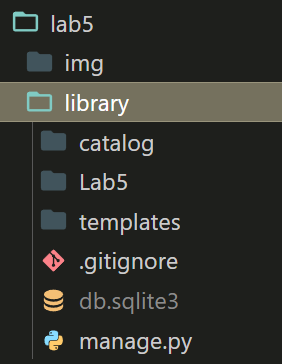
\includegraphics[scale=0.5]{img/img0.png}
        \caption{Estructura de proyecto}
        \label{fig:imagen}
    \end{figure}
    
    \begin{figure}[H]
        \centering
        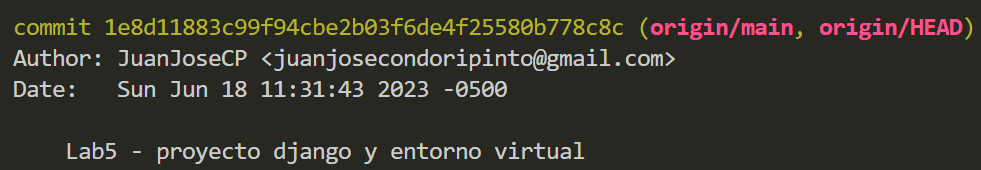
\includegraphics[scale=0.5]{img/img0_commit.png}
        \caption{Primer commit para creación de estructura de proyecto}
        \label{fig:imagen}
    \end{figure}

    Luego de haber creado el proyecto, lo siguiente será ejecutar las migraciones que vienen por defecto dentro de django, así como añadir dentro de models.py las clases de modelo que usaremos para el resto del proyecto.

	\begin{lstlisting}[language=bash,caption={Realizando migraciones}][H]
		$ python manage.py makemigrations
            $ python manage.py migrate
	\end{lstlisting}

    \begin{figure}[H]
        \centering
        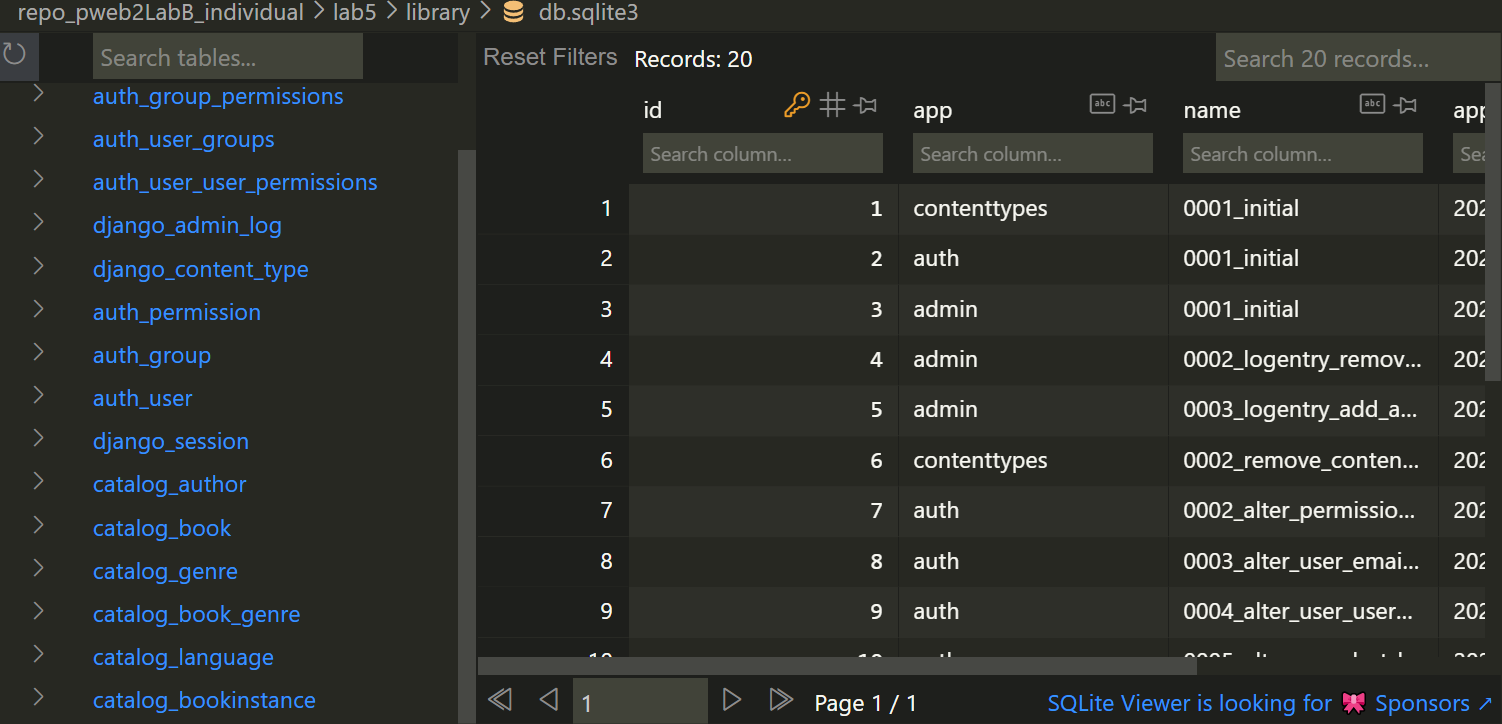
\includegraphics[scale=0.5]{img/img1.png}
        \caption{Tablas de sqlite3 luego de migración}
        \label{fig:imagen}
    \end{figure}

    \begin{figure}[H]
        \centering
        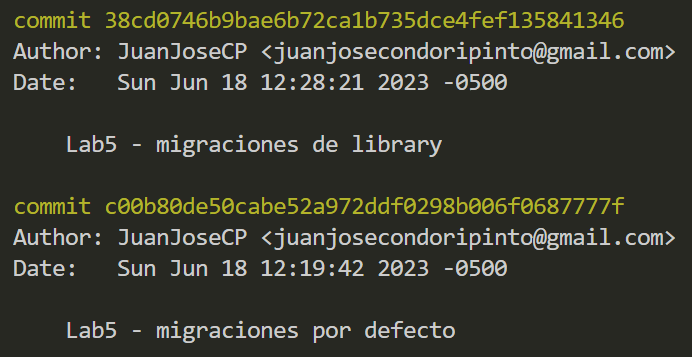
\includegraphics[scale=0.5]{img/img1_commit.png}
        \caption{Commit para migraciones de django y modelos library}
        \label{fig:imagen}
    \end{figure}

    Una vez creadas las migraciones para la base de datos, procedemos a crear un superusuario e iniciar el servidor para acceder a la vista de administrador.

	\begin{lstlisting}[language=bash,caption={Creando superusuaio y corriendo el servidor}][H]
		$ python manage.py createsuperuser
            $ python manage.py runserver
	\end{lstlisting}

    \begin{figure}[H]
        \centering
        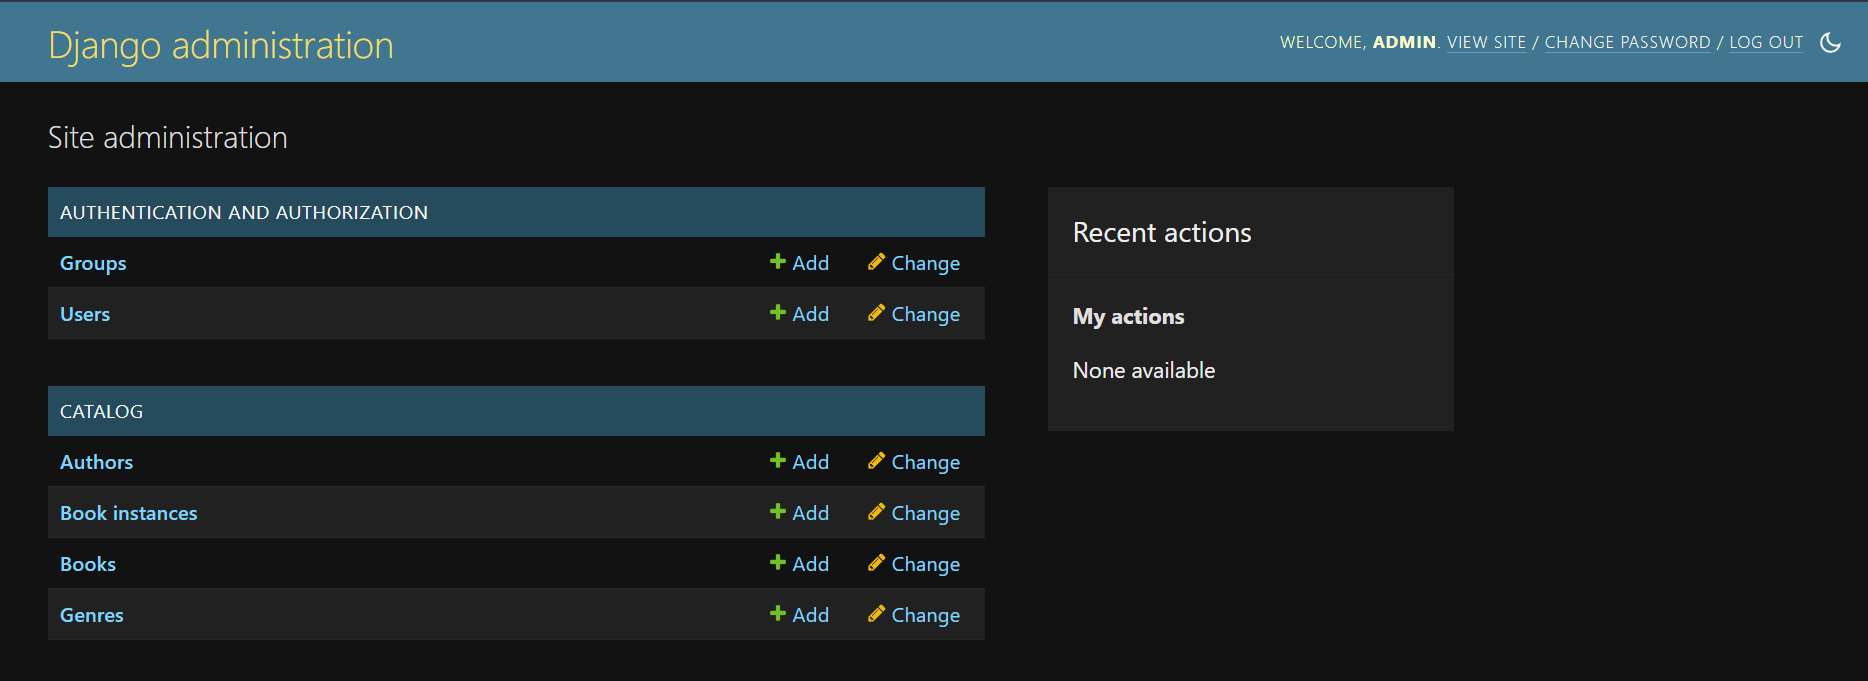
\includegraphics[scale=0.42]{img/img2.png}
        \caption{Vista de administrador}
        \label{fig:imagen}
    \end{figure}

    \begin{figure}[H]
        \centering
        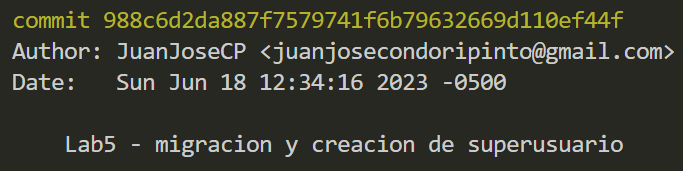
\includegraphics[scale=0.5]{img/img2_commit.png}
        \caption{Commit para creación de superusuario}
        \label{fig:imagen}
    \end{figure}

    Cuando registramos los modelos dentro de admin.py en nuestra aplicación de catalog, automaticamente estos pasan a ser campos modificables dentro de la vista de administrador:

    \begin{figure}[H]
        \centering
        
\includegraphics[scale=0.42]{img/img3.png}
        \caption{Vista admin para la modificación de autores (lista)}
        \label{fig:imagen}
    \end{figure}

    \begin{figure}[H]
        \centering
        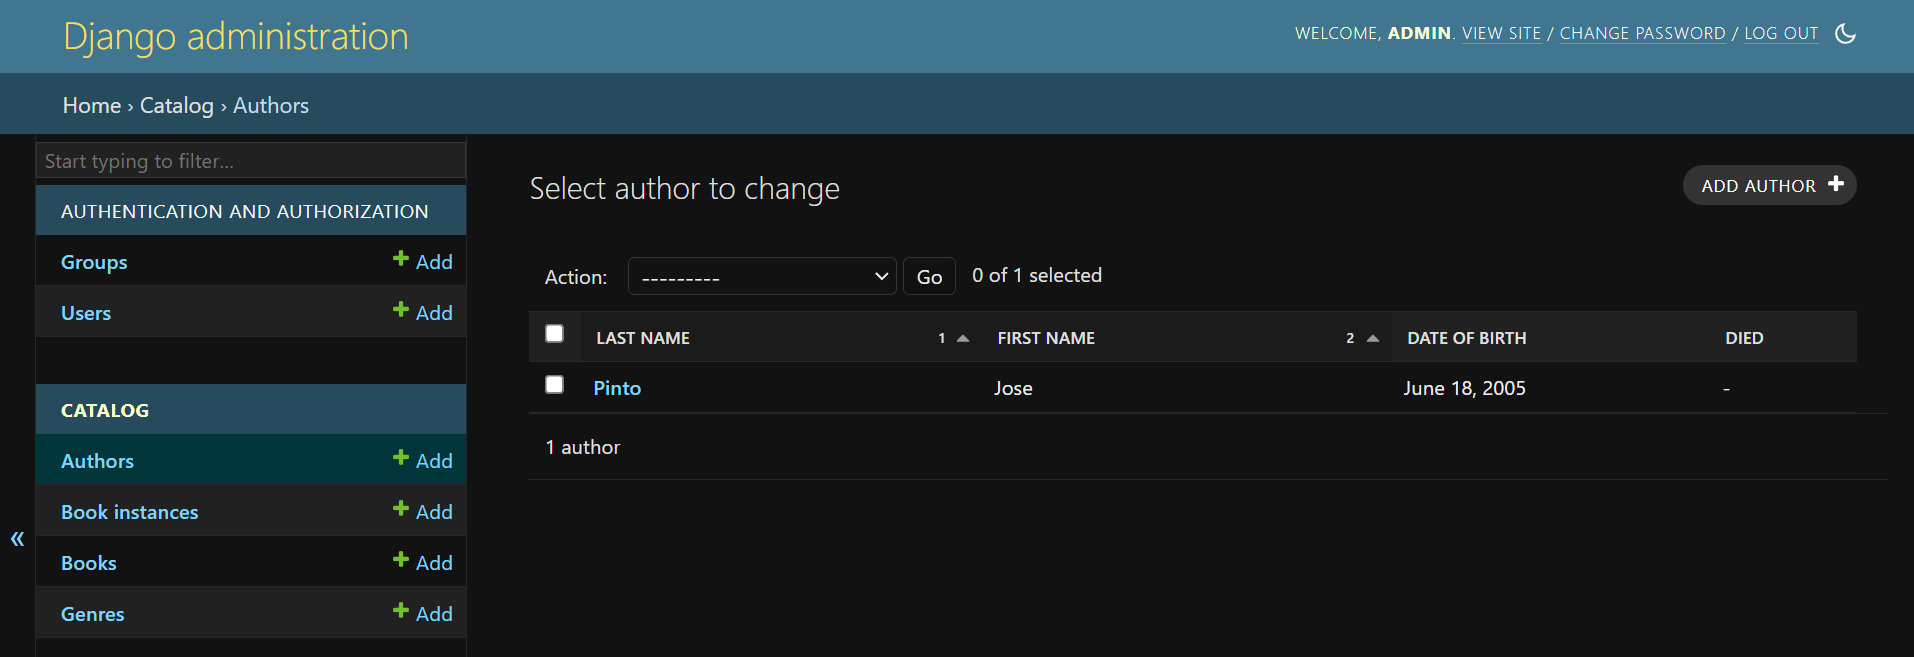
\includegraphics[scale=0.42]{img/img4.png}
        \caption{Tabla de autores luego de añadir list-display en admin.py}
        \label{fig:imagen}
    \end{figure}

    \begin{figure}[H]
        \centering
        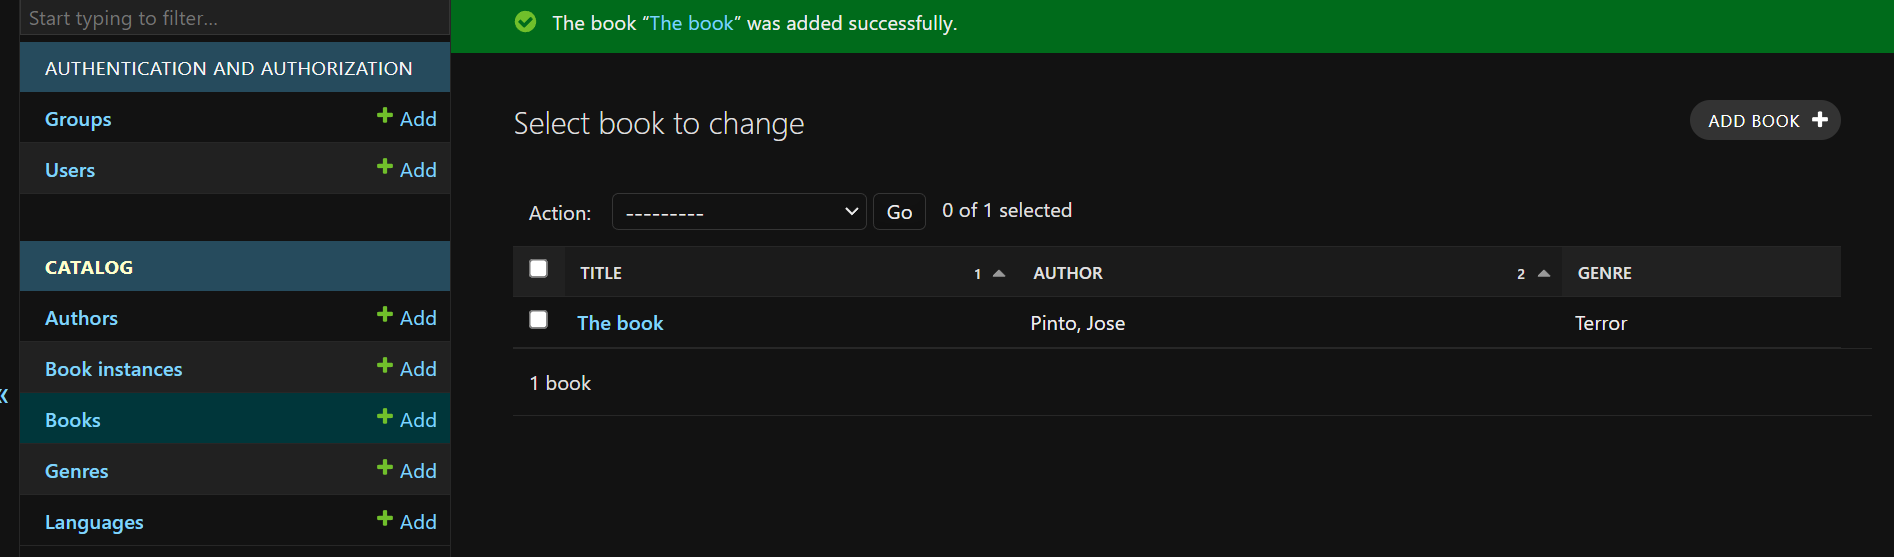
\includegraphics[scale=0.42]{img/img5.png}
        \caption{Tabla de libros para vista de admin}
        \label{fig:imagen}
    \end{figure}

    \begin{figure}[H]
        \centering
        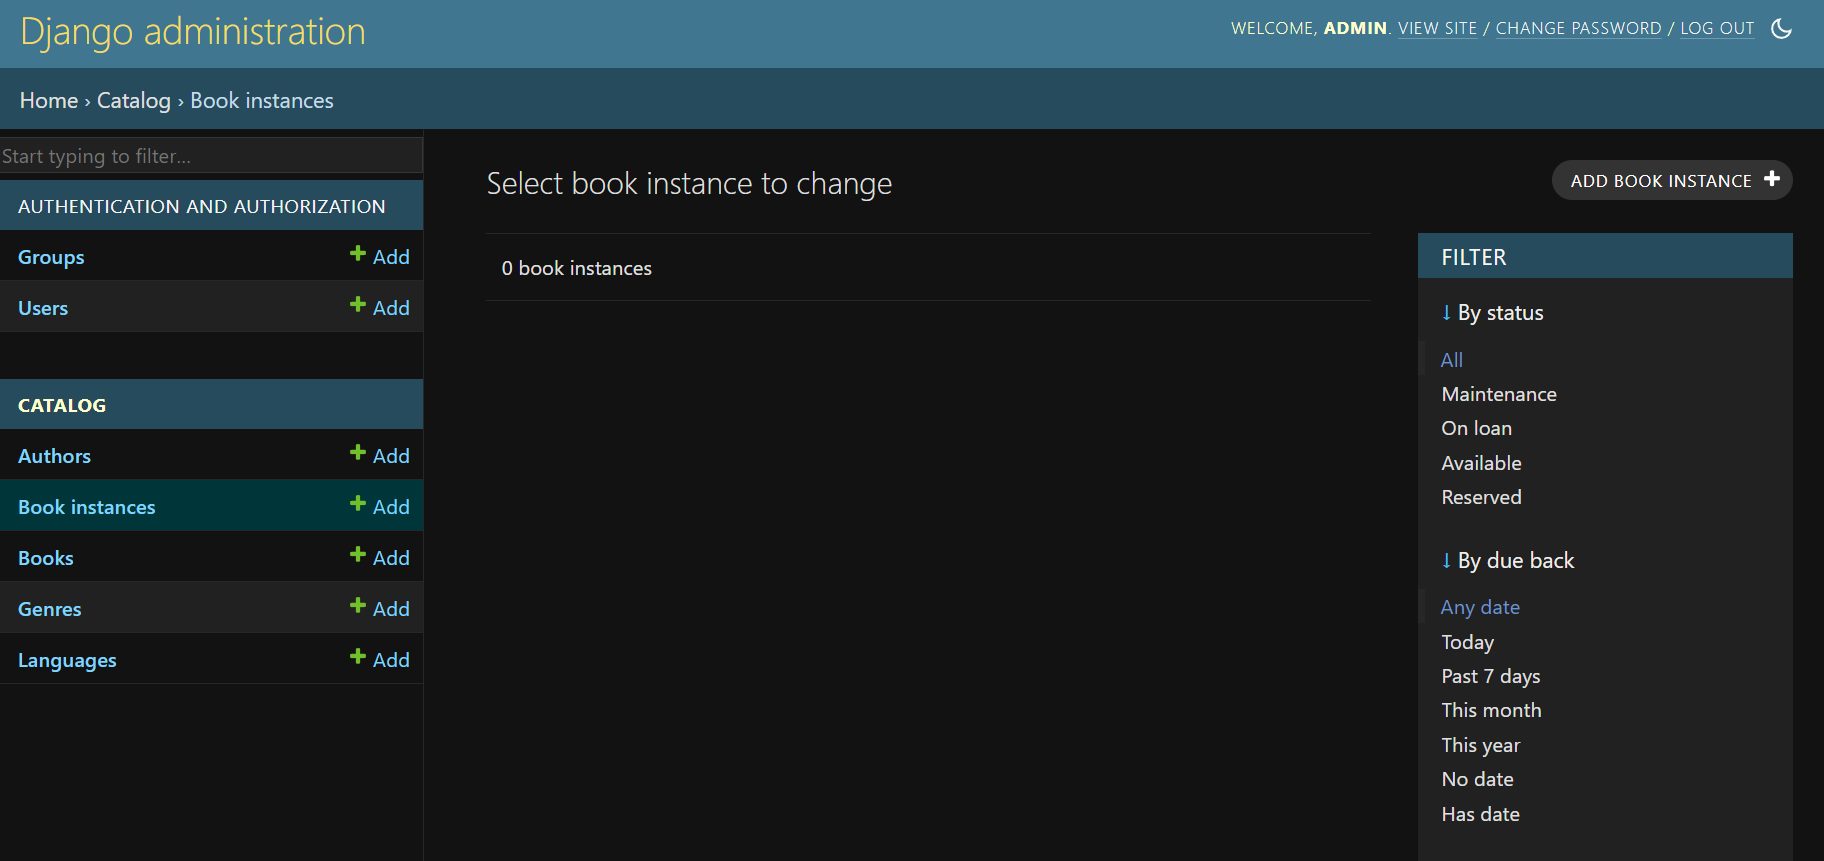
\includegraphics[scale=0.42]{img/img6.png}
        \caption{Campo de filtros para tabla de libros}
        \label{fig:imagen}
    \end{figure}
    
    \begin{figure}[H]
        \centering
        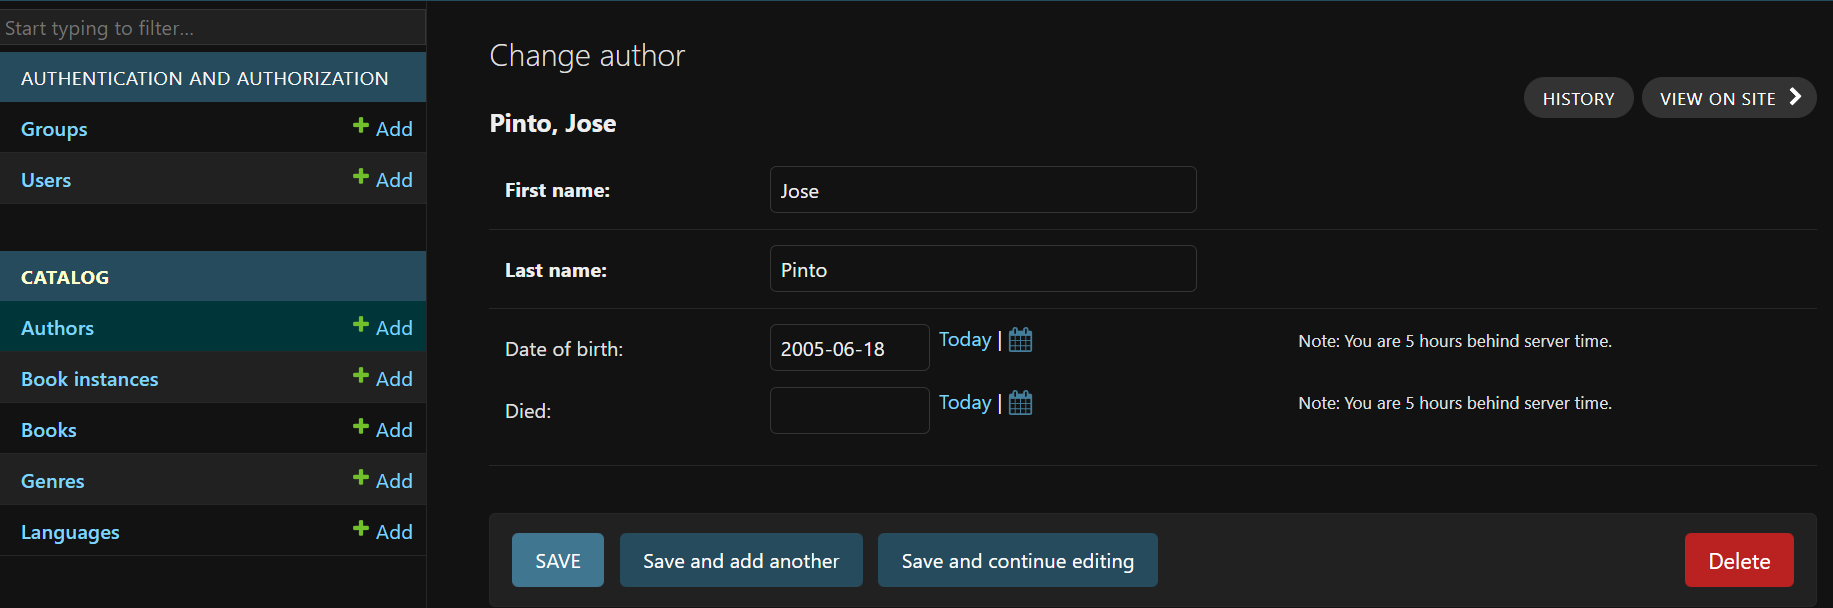
\includegraphics[scale=0.42]{img/img7.png}
        \caption{Vista de autor para modificación de campos}
        \label{fig:imagen}
    \end{figure}

    \begin{figure}[H]
        \centering
        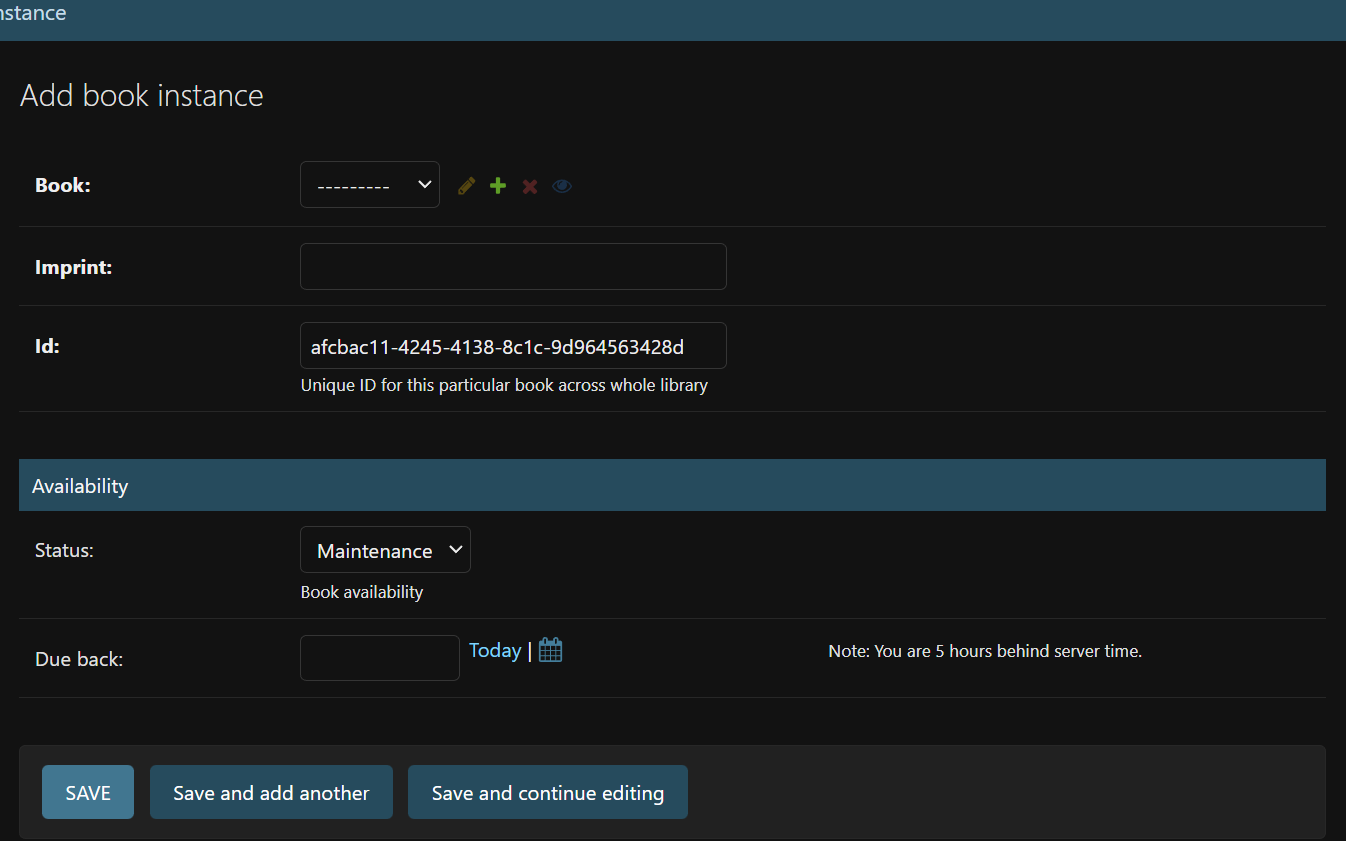
\includegraphics[scale=0.42]{img/img8.png}
        \caption{Modificación de instancia de libro}
        \label{fig:imagen}
    \end{figure}

    \begin{figure}[H]
        \centering
        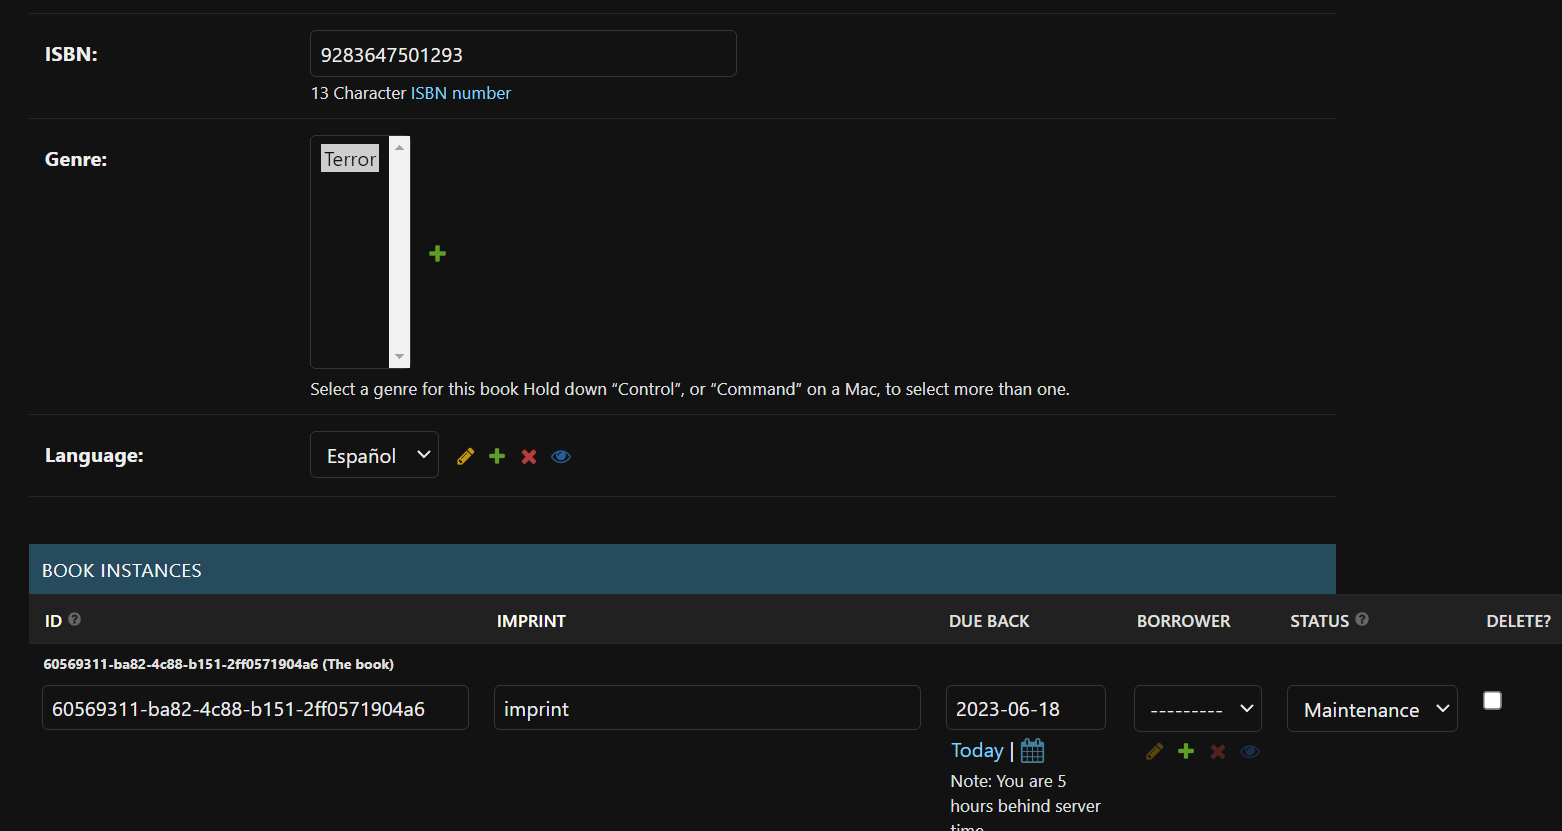
\includegraphics[scale=0.42]{img/img9.png}
        \caption{Vista de tabla de instancias de libro horizontal en parte inferior de libro}
        \label{fig:imagen}
    \end{figure}

    \begin{figure}[H]
        \centering
        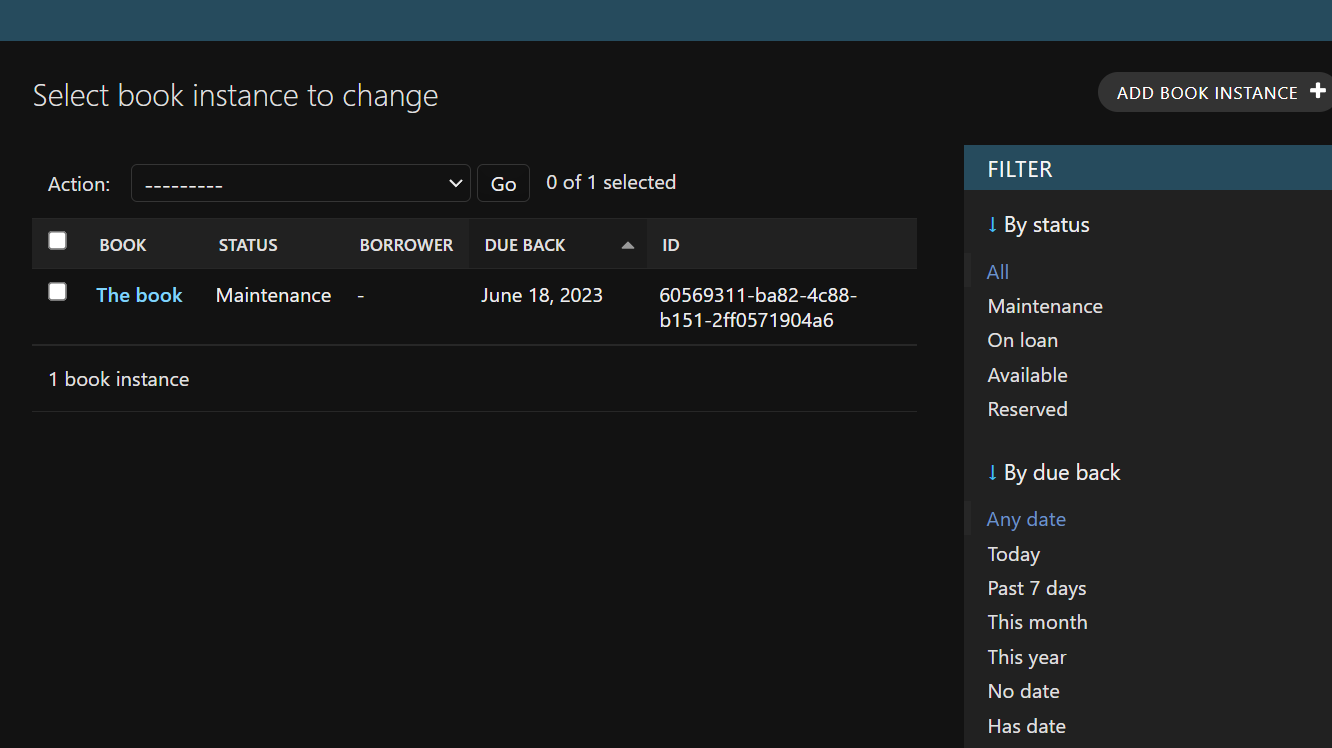
\includegraphics[scale=0.42]{img/img10.png}
        \caption{Vista de tabla de instancias de libros}
        \label{fig:imagen}
    \end{figure}

    Las vistas del administrador son para la interacción directa con la base de datos, sin embargo, para el proyecto de library son requeridas otras vistas más específicas para su disposición al usuario, es por ello que dentro de la aplicación fueron creadas varias plantillas en jinja, ello permitió la herencia de componentes, reutilización y aplicación de objetos y variables pasadas por el backend:

    La estructura del proyecto se amplió algo más, ya que para cada vista se requiere una acción en concreto de nuestros controladores.

    \begin{figure}[H]
        \centering
        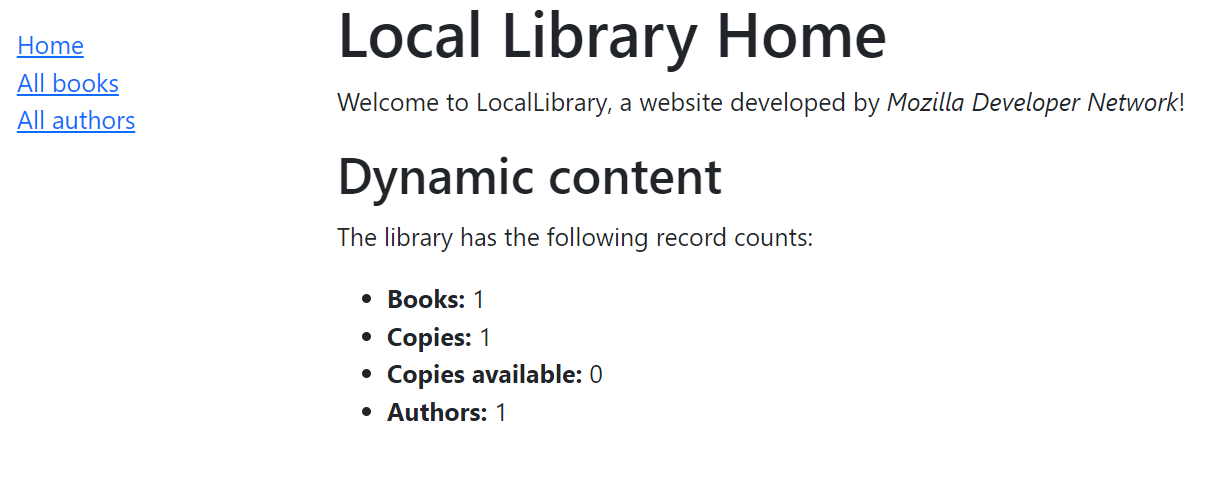
\includegraphics[scale=0.42]{img/img11.png}
        \caption{Vista index de aplicación catalog}
        \label{fig:imagen}
    \end{figure}

    \begin{figure}[H]
        \centering
        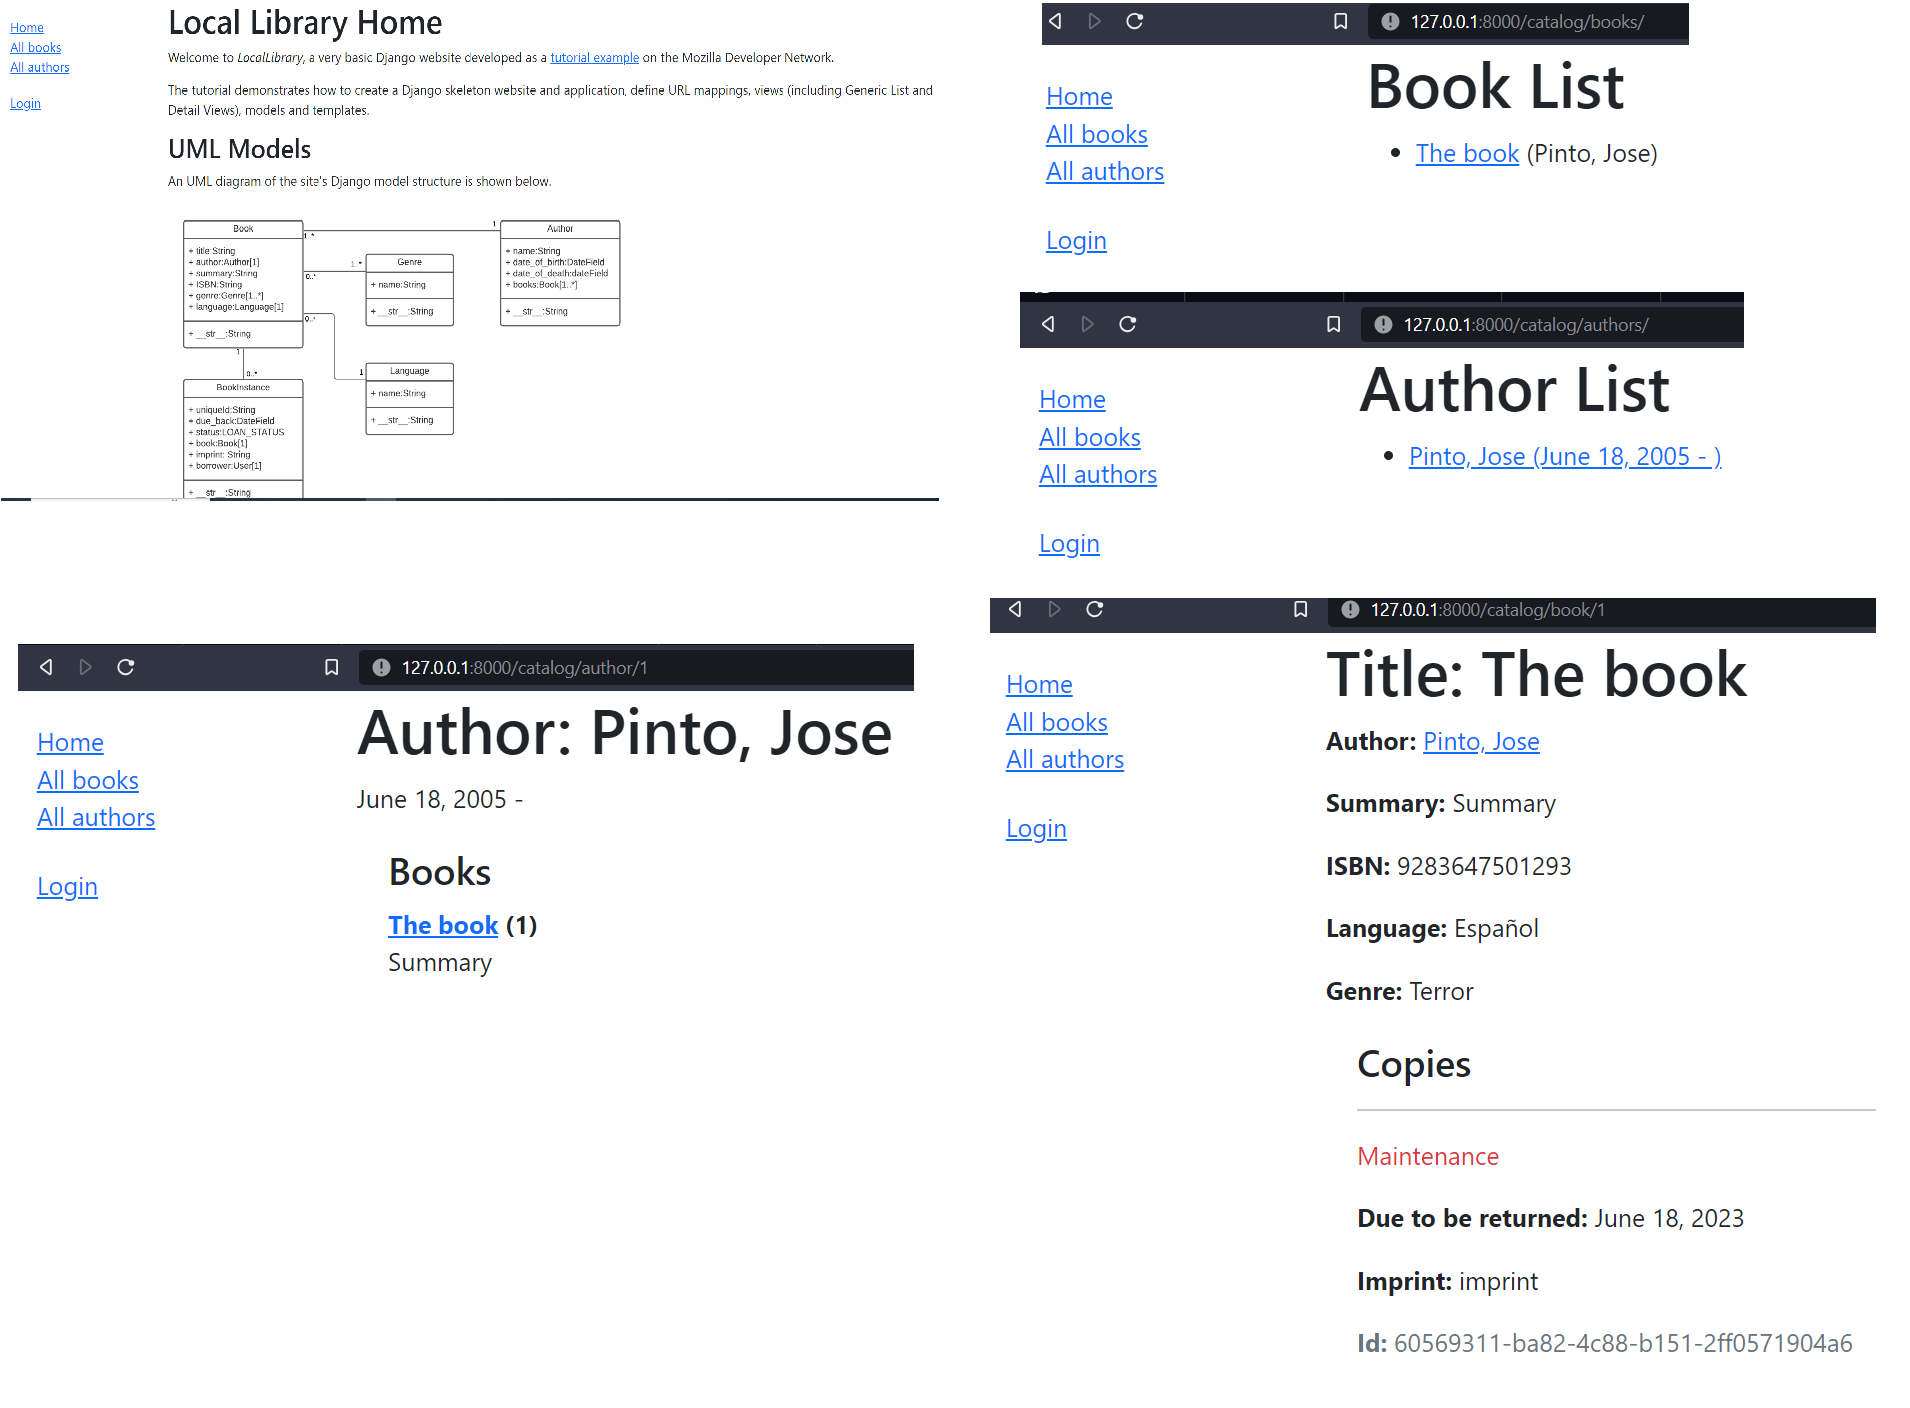
\includegraphics[scale=0.42]{img/img12.png}
        \caption{Acciones dentro de vistas de libros y autores}
        \label{fig:imagen}
    \end{figure}

    \begin{figure}[H]
        \centering
        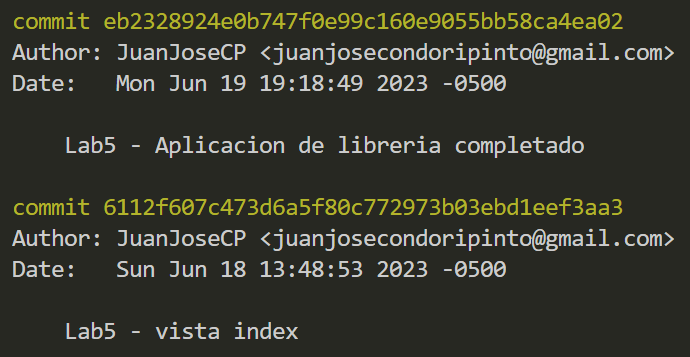
\includegraphics[scale=0.42]{img/img11_commit.png}
        \caption{Commmit para vistas y aplicación de catalog}
        \label{fig:imagen}
    \end{figure}

    \section{Trabajo final}
        La aplicación que se estará trabajando el resto del semestre tiene como base el manejo y gestión de un negocio (no se especifica el tipo), donde el usuario tendrá la capacidad de manejar los aspectos más básicos tales como empleados, ingresos, egresos, reportes, etc.

    \section{Pregunta}
        \begin{itemize}
            \item Por cada integrante del equipo, resalte un aprendizaje que adquirio al momento de estudiar Django. No se reprima de ser detallista. Coloque su nombre entre parentesis para saber que es su aporte.
        \end{itemize}
        (Juan José Condori Pinto) Aprendí los conceptos básicos de django, su distribución, arquitectura y utilidad para el desarrollo de aplicaciones web desde el back end con python, lo cual, agiliza su implementación al ser este un lenguaje flexible y débilmente tipado; aprendí sobre los conceptos básicos de enrutamiento, migraciones a bases de datos locales y manejo de datos a través de plantillas o desde el front; sin embargo, comprendí que Django es un framework que se orienta algo más para el backend, por lo cual, el uso de plantillas no está mal, pero es más efectivo el uso de otras herramientas para su diseño, dejando Django para el lado del servidor y disposicion de apis.
        
    \section{\textcolor{red}{Rubricas}}
        \subsection{\textcolor{red}{Rubrica para entregable Informe}}
            \begin{table}[ht]
                \centering
                \caption{Rúbrica para tipo de informe}
                \begin{tabular}{
                        |p{2.5cm}
                        |p{6cm}
                        |p{2cm}
                        |p{2cm} |}
                    \hline
                        \multicolumn{2}{|c|}{\textbf{Informe}} & \centerline{\textbf{Cumple}} & \centerline{\textbf{No cumple}} \\
                    \hline
                        \textbf{\textcolor{red}{Latex}} & \textcolor{blue}{El informe esta en formato PDF desde Latex, con un formato limpio (buena presentación) y facil de leer.} & \centerline{20} & \centerline{0} \\
                    \hline
                        \textbf{MarkDown} & El informe esta en formato PDF desde MarkDown README.md, con un formato limpio (buena presentacion) y facil de leer. & \centerline{17} & \centerline{0}\\
                    \hline
                        \textbf{MS Word} & El informe esta en formato PDF desde plantilla MS Word, con un formato limpio (buena presentacion) y facil de leer. & \centerline{15} & \centerline{0}\\
                    \hline
                        \textbf{Observaciones} & Por cada observacion se le descontara puntos. & \centerline{-} & \centerline{-}\\
                    \hline
                    \end{tabular}
                \label{tab:tab1}
            \end{table}
        \subsection{\textcolor{red}{Rubrica para el contenido del Informe y demostracion}}
            \begin{itemize}
                \item El alumno debera marcar o dejar en blanco en las celdas de la columna Checklist, deacuerdo a si cumplio o no con el ́ıtem correspondiente.
                \item Si un alumno supera la fecha de entrega, su calificacion siempre sera sobre la nota mınima aprobada, siempre y cuando cumpla con todos lo items.
                \item El alumno debe autocalificarse en la columna Estudiante de acuerdo a la tabla de calificacion de niveles de desempeño:
            \end{itemize}
            \begin{table}[ht]
                \centering
                \caption{Niveles de desempeño}
                \begin{tabular}{
                        >{\centering\arraybackslash}m{1.2cm}
                        >{\centering\arraybackslash}m{3cm}
                        >{\centering\arraybackslash}m{3cm}
                        >{\centering\arraybackslash}m{3cm}
                        >{\centering\arraybackslash}m{3cm}}
                    \hline
                    \multicolumn{5}{c}{Nivel} \\
                    \hline
                    \textbf{Puntos} & Insatisfactorio 25\% & En Proceso 50\% & Satisfactorio 75\% & Sobresaliente 100\% \\
                    \textbf{2.0} & 0.5 & 1.0 & 1.5 & 2.0 \\
                    \textbf{4.0} & 1.0 & 2.0 & 3.0 & 4.0 \\
                    \hline
                \end{tabular}
                \label{tab:tab2}
            \end{table}
            \begin{table}[]
                \centering
                \caption{Rubrica para contenido del Informe y demostracion}
                \begin{tabular}{
                    |m{2.5cm}
                    |m{7cm}
                    |>{\centering\arraybackslash}m{1cm}
                    |>{\centering\arraybackslash}m{1.2cm}
                    |>{\centering\arraybackslash}m{1.5cm}
                    |>{\centering\arraybackslash}m{1.2cm}|}
                    
                    \hline
                    \multicolumn{2}{|c|}{Contenido y demostracion} & Puntos & Checklist & Estudiante & Profesor \\
                    \hline
                    \textbf{1. GitHub} & Hay enlace URL activo del directorio para el laboratorio hacia su repositorio GitHub con codigo fuente terminado y facil de revisar. & 2 & X & 2 &   \\
                    \hline
                    \textbf{2. Commits} & Hay capturas de pantalla de los commits mas importantes con sus explicaciones detalladas. (El profesor puede preguntar para refrendar calificacion). & 4 & X & 3 &   \\
                    \hline
                    \textbf{3. Código fuente} & Hay porciones de codigo fuente importantes con numeracion y explicaciones detalladas de sus funciones. & 2 & X & 1.5 &   \\
                    \hline
                    \textbf{4. Ejecucion} & Se incluyen ejecuciones/pruebas del codigo fuente explicadas gradualmente. & 2 & X & 1 &   \\
                    \hline
                    \textbf{5. Pregunta} & Se responde con completitud a la pregunta formulada en la tarea. (El profesor puede preguntar para refrendar calificacion). & 2 & X & 2 &   \\
                    \hline
                    \textbf{6. Fechas} & Las fechas de modificacion del codigo fuente estan dentro de los plazos de fecha de entrega establecidos. & 2 & X & 1 &   \\
                    \hline
                    \textbf{7. Ortografia} & El documento no muestra errores ortograficos. & 2 & X & 2 &   \\
                    \hline
                    \textbf{8. Madurez} & El Informe muestra de manera general una evolucion de la madurez del codigo fuente, explicaciones puntuales pero precisas y un acabado impecable. (El profesor puede preguntar para refrendar calificacion). & 4 & X & 2 &   \\
                    \hline
                    
                \end{tabular}
                \label{tab:tab3}
            \end{table}
    \section{Referencias}
        \begin{itemize}
            \item \url{https://developer.mozilla.org/en-US/docs/Learn/Server-side/Django/Tutorial_local_library_website}
            \item \url{https://github.com/mdn/django-locallibrary-tutorial}
            \item \url{https://github.com/rescobedoq/pw2/tree/main/labs/lab05}
            \item William S. Vincent. (2022). Django for Beginners: Build websites with Python. Django 4.0.leanpub.com [\href{http://library.lol/main/22AF742D96697DE55EF5F88B08F1AA86}{URL}]
            \item \url{https://docs.djangoproject.com/en/4.1/ref/models/fields/}
            \item \url{https://docs.djangoproject.com/en/4.0/topics/db/examples/many_to_many/}
            \item \url{https://docs.djangoproject.com/en/4.0/topics/db/examples/many_to_one/}
            \item \url{https://blog.hackajob.co/djangos-new-database-constraints/}
            \item \url{https://stackoverflow.com/questions/3330435/is-there-an-sqlite-equivalent-to-mysqls-describe-table}
            \item \url{https://docs.djangoproject.com/en/4.1/ref/validators/#how-validators-are-run}
            \item \url{https://docs.djangoproject.com/en/4.1/ref/models/instances/}
        \end{itemize}
\end{document}